
\section*{Psi}
\DefineNamedColor{named}{eclipsered}{rgb}{0.586,0.466,0.682}
\definecolor{tablecolor}{named}{eclipsered}

\subsection*{Invoking}

\begin{figure}[H]%
   \centering
   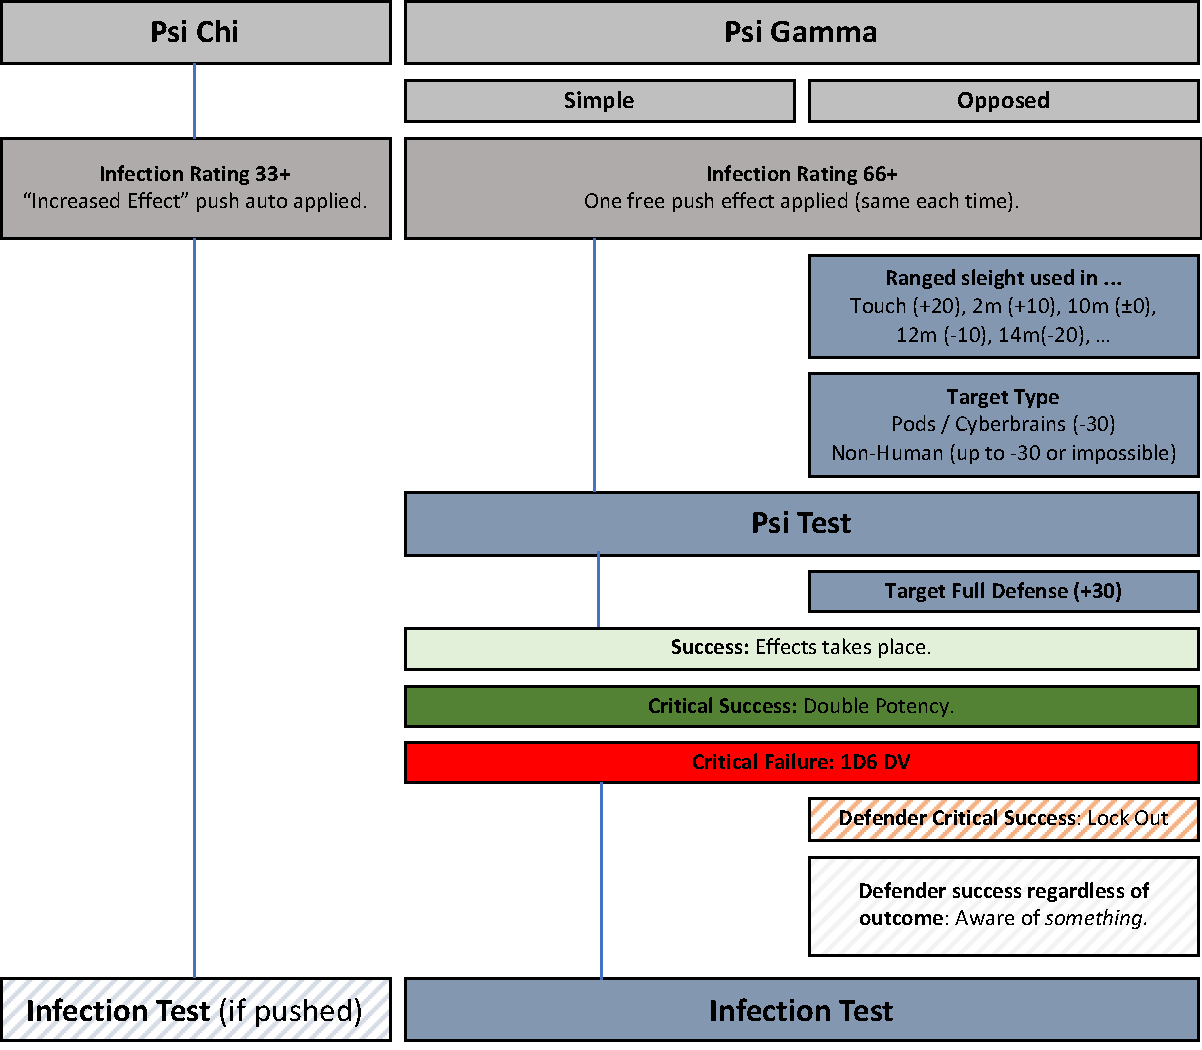
\includegraphics[scale=0.615]{gfx/psi-flow}%
\end{figure}%

\bigskip

\begin{eptable}{ l | X }
   \epheader{2}{Targeting}
   Multiple Targets & Single roll vs. multiple opposed. IR \modifier{+5} per target more.\\
   Animals & Partially sapient \modifier{-20}, non-sapient animals \modifier{-30}.\\
   Aliens & At least \modifier{-20}, might not work at all.\\
\end{eptable}

\bigskip

\begin{eptable}{ l | X }
   \epheader{2}{Psi-Gamma ranged ability used in ...}
   Touch & Gives \modifier{+20} if in physical contact.\\
   Point Blank & Gives  \modifier{+10}, if within \SI{2}{m}.\\
   Close & Must be within \SI{10}{m}, \modifier{-10} for each \SI{2}{m} beyond.\\
   Psi vs Psi & Ranges double against other async.\\
\end{eptable}


\bigskip

\begin{eptable}{ l | X }
   \epheader{2}{Duration}
   Constant & Always on.\\
   Instant & Immediate and permanent.\\
   Temporary & Lasts \skill{WIL} / 5 time units, as defined in sleight.\\
   Sustained & Requires concentration, \modifier{-10} to Async for duration.\\
\end{eptable}

\begin{itemize}
    \itembox Multiple sleights might be sustained with each incurring additional \modifier{-10}.
    \itembox Async must also stay within range.
\end{itemize}

\bigskip

\begin{eptable}{ l | X }
   \epheader{2}{Pushing Sleights}
    Increase Range & Touch becomes Close, Close \SI{20}{m}, Close (Async) \SI{30}{m}.\\
    Increase Effect & Any modifiers are doubled.\\
    Increase Power & Resisted by \skill{WIL}\,/\,2 instead of \skill{WIL}.\\
    Increase Penetration & Psi Shield reduced by half.\\
    Increase Duration & Double duration (temporary sleights only).\\
    Extra Target & Target extra victim with same action.\\
\end{eptable}

\begin{itemize}
    \itembox \textbf{Doubles Infection Rating} when pushing. User also suffers \dv{1d6}.
    \itembox \textbf{Psi-Chi Pushing}. Infection rating raises by \num{5} and causes Infection test. Boosting them lasts for \skill{WIL}\,/\,\SI{5}{min}.
    \itembox \textbf{Moxie} to avoid making Infection costs \num{2} if pushed.
\end{itemize}


\bigskip

\subsection*{Infection Test}


\begin{figure}[H]%
   \centering
   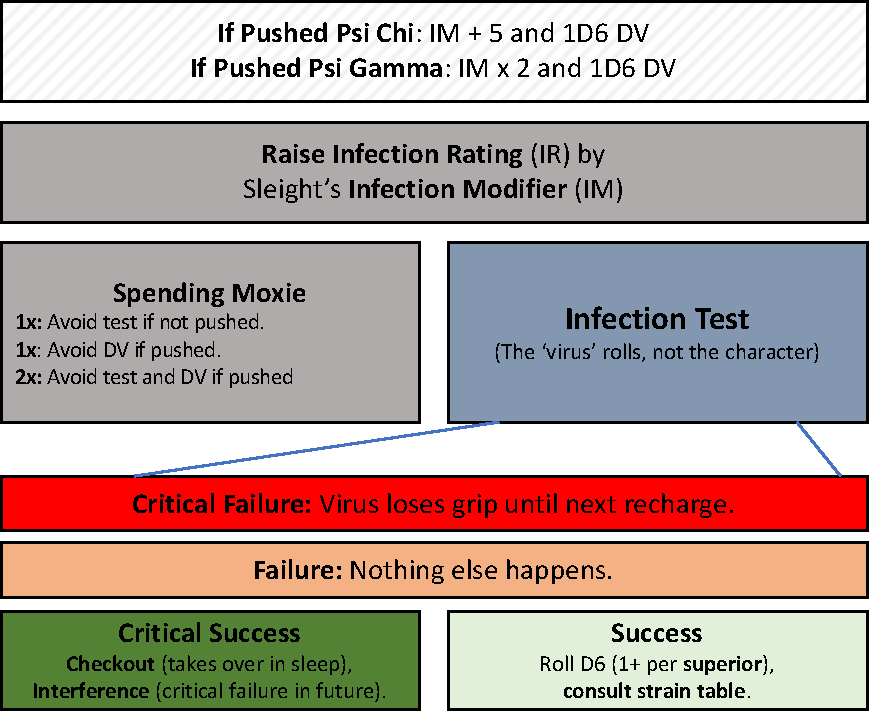
\includegraphics[scale=0.615]{gfx/psi-infection}%
\end{figure}%

\bigskip

\begin{itemize}
    \itembox \textbf{Role Playing}. Consider have other player do Infection Test, and role play the \textit{voice of the infection}, describe compulsions and hallucinations, or even maintain a sort of alter-ego internal dialogue with the async.
    \itembox \textbf{Checkout Time}. Next long rest or unconscious situation infection may take over and acts with character without character knowing.
    \itembox \textbf{Interference}. When in future making some test, do an opposed \skill{WIL} vs. \skill[+30]{Infection} before that. If infection wins, player suffers critical failure. Preferably during dramatic situations.
    \itembox Each short rest reduces Infection Rating by \modifier{-10} (down to base). Each long rest resets Infection Rating to base.
\end{itemize}

\bigskip

\begin{eptable}{ l | X }
   \epheader{2}{Infection Rating Thresholds}
   IR 33+ & Increased Effect push automatically active.\\
   IR 66+ & Additional free push unlocked and automatically active.\\
\end{eptable}

\bigskip

\begin{eptable}{ l | X }
   \epheader{2}{General Strain Effects}
   Physical Damage & Suffer \dv{1d6} as fatigue, headache, hemorrhaging.\\
   Modified Behavior & Change behavior for \dice{1d6} minutes, severity based on IR.\\
   Motivation & For \dice{1d6} hours, get motivation.\\
\end{eptable}

\begin{itemize}
   \itembox \textbf{Modified Behavior}. If IR $<$ 33 player is compelled to perform or avoid. If IR $<$ 66 a \skill{WIL} check is needed. If IR $\geq$ 66 also suffer \dice{1d6} stress if not complying.
   \itembox \textbf{Motivation}. If role played played well, recover stress. If not fulfilled, receive \dice{1d6} stress. Resisting motivation requires \skill{WIL} and inflicts \modifier{-10} to all actions.
\end{itemize}

\bigskip

\begin{eptable}{ l | X }
   \epheader{2}{Architect Sub-Strain}
   1 & Physical Damage, \dv{1d6} as fatigue, headache, hemorrhaging.\\
   2 & Enhanced Behavior: Arrogance.\\
   3 & Restricted Behavior: Relaxation.\\
   4 & Motivation: +Hoard (hoard weird things, organs, \textellipsis).\\
   5 & Motivation: +Expose Inner (open, dissect, \textellipsis).\\
   6 & Motivation: +Create (create something weird, \textellipsis).\\
\end{eptable}

\bigskip

\begin{eptable}{ l | X }
   \epheader{2}{Beast Sub-Strain}
   1 & Physical Damage, \dv{1d6} as fatigue, headache, hemorrhaging.\\
   2 & Enhanced Behavior: Aggression.\\
   3 & Restricted Behavior: Remorse.\\
   4 & Motivation: +Domination (do whatever needed to win).\\
   5 & Motivation: +No Quarter (don't flee, surrender).\\
   6 & Frenzy (rage if blood spilled, prefer melee, \ldots).\\
\end{eptable}

\bigskip

\begin{eptable}{ l | X }
   \epheader{2}{Haunter Sub-Strain}
   1 & Physical Damage, \dv{1d6} as fatigue, headache, hemorrhaging.\\
   2 & Enhanced Behavior: Avoidance.\\
   3 & Enhanced Behavior: Mistrust.\\
   4 & Motivation: +Cut Ties (relationships are pointless).\\
   5 & Motivation: +Isolation (truly go, commune with dark void).\\
   6 & Hallucination (for \SI{24}{h} experience hallucinations).\\
\end{eptable}

\bigskip

\begin{eptable}{ l | X }
   \epheader{2}{Stranger Sub-Strain}
   1 & Physical Damage, \dv{1d6} as fatigue, headache, hemorrhaging.\\
   2 & Enhanced Behavior: Deceit.\\
   3 & Enhanced Behavior: Self Sabotage.\\
   4 & Motivation: +Foil Plans (make others fail in their plans).\\
   5 & Motivation: +Manipulation (make others fit into your plans).\\
   6 & Motivation: +Test Limits (push horrible boundaries).\\
\end{eptable}

\bigskip

\begin{eptable}{ l | X }
   \epheader{2}{Xenomorph Sub-Strain}
   1 & Physical Damage, \dv{1d6} as fatigue, headache, hemorrhaging.\\
   2 & Enhanced Behavior: Non-verbal Communication.\\
   3 & Enhanced Behavior: Cliquishness.\\
   4 & Motivation: +Transform Environment (for alien presence).\\
   5 & Motivation: +Control Territory (set traps, protect from intruders).\\
   6 & Motivation: +Express True Form (modify yourself to true form).\\
\end{eptable}

Sub-strain effect list is gross oversimplification. Check rule book for detailed advice how strain acts and how to role play.
